% Chapter 4

\chapter{Travaux et apports} % 4th chapter title

\label{Chapter4} % For referencing the chapter elsewhere, use \ref{Chapter4} 


%----------------------------------------------------------------------------------------


\section{Les missions du poste}

\begin{itemize}
    \item L'état de l'art de la partie précédente fait partie des missions.
    \item Modélisation
    \item Simulation
\end{itemize}

Nous souhaitons étudier le comportement mécanique d'un floe après collision avec un autre floe. Les étapes de travail envisagées sont les suivantes:
\begin{enumerate}
    \item Ecire les systèmes differentiels pour les deux floes juste après le choc: pour l' instant on peut considérer que l'un des floes est immobile (celà revient au même si l'on exprimes les vitesses dans un repère lié à ce floe).
    \item On exprime l'EDO vérifiée par les solutions, c'est à dire $q$ pour le premier floes, et $p$ pour le second.
    \item On pourra ensuite simuler ces EDP limites et trouver les valeurs de $p$ et $q$. Autrement dit, on connait la position de chaque point du réseau au temps final.
    \item Si on connait $p$ et/ou $q$, on connait la condition de Dirichlet sur le floe concerné, et on peut ainsi exprimer le déplacement et la possible fracture du floe. 
\end{enumerate}







\section{Présentation des résultats obtenus}










\subsection{Modélisation et simulation 1D}









\subsubsection{Modélisation du déplacement d'un floe isolé}

Avant d'entamer la question de la percussion, étudions le comportement d'un floe de glace 1D modélisé par un réseau de ressorts (1 ressort, 1 dispositif viseux, et 2 noeuds) (voir \cref{fig:deplacement1d}).
\begin{figure}[!h]
    \centering
    \frame{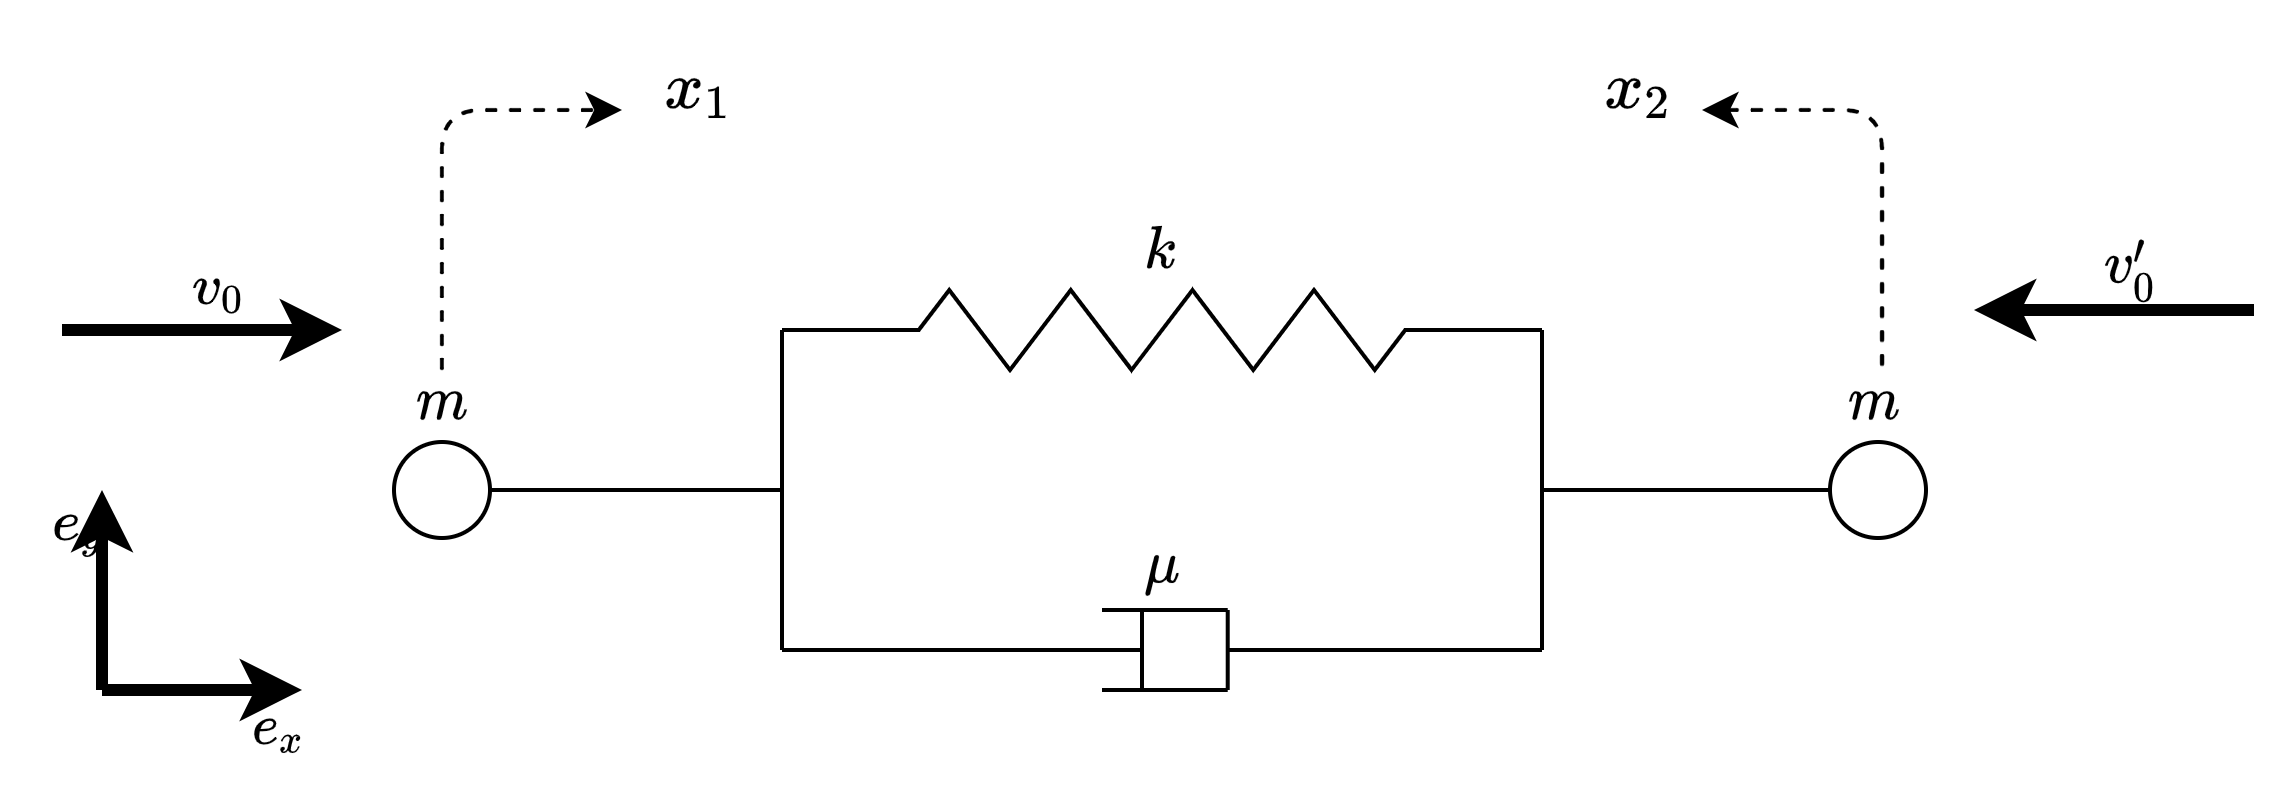
\includegraphics[width=0.6\textwidth]{Deplacement1D-Systeme.png}}
    \caption{Floe de glace 1D modélisé par un réseau de ressorts. Le floe est isolé de toutes forces extérieurs. Les varaibles $x_1$ et $x_2$ traduisent les déplacemnts des noeuds de gauche et de droite respectifs. À l'instant initial, les masses sont soumises aux vitesses $v_0$ et $v'_0$ indiquées.}
    \label{fig:deplacement1d}
\end{figure}


\begin{figure}[!h]
    \begin{subfigure}[b]{0.33\textwidth}
        \centering
        \frame{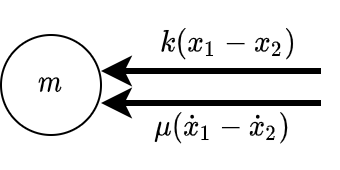
\includegraphics[width=\textwidth]{Deplacement1D-Masse1.png}}
        \caption{Sur la masse $m$ de gauche.}
    \end{subfigure}
%     \hfill
    \begin{subfigure}[b]{0.3\textwidth}
        \centering
        \frame{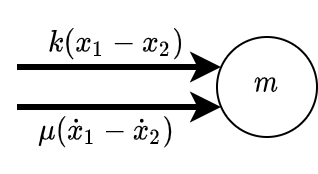
\includegraphics[width=\textwidth]{Deplacement1D-Masse2.png}}
        \caption{Sur la masse $m$ de droite.}
    \end{subfigure}
       \caption{Bilan des forces appliquée sur les noeuds du système. Les valeurs indiquées sont les intensitées (positives) des forces (par exemple juste après l'instant initial, on a $x_1 > 0$, et $x_2 < 0$ d'où $k(x_1-x_2) > 0$).}
       \label{fig:bilan0}
\end{figure}


\noindent Un bilan des forces effectué sur les deux noeuds du floe (voir \cref{fig:bilan0}) permet d'obtenir les équations suivantes:
\begin{align}
    \begin{dcases}
    m\ddot x_1 = - k(x_1 - x_2) - \mu(\dot x_1 - \dot x_2) \,,\\
        m \ddot x_2 =  k(x_1 - x_2) + \mu(\dot x_1 - \dot x_2) \,. 
    \end{dcases}
\end{align}
En remarquant que $m\neq 0$, on passe à la forme matricielle qui s'écrit:
\begin{align}
    \myvec{\ddot{x}_1}{\ddot{x}_2} = 
      \underbrace{ \frac{k}{m} \mymat{-1}{1}{1}{-1}}_{B} \myvec{x_1}{x_2}
    + \underbrace{\frac{\mu}{m} \mymat{-1}{1}{1}{-1}}_{C} \myvec{\dot{x}_1}{\dot{x}_2} \,.
\end{align}
On pose ensuite la matrice par blocs:
\[ E = \mymat{0}{I_2}{B}{C}  =  \begin{pmatrix}
    0 & 0 & 1 & 0 \\ 0 & 0& 0& 1 \\ -\frac{k}{m} & \frac{k}{m} & -\frac{\mu}{m} & \frac{\mu}{m} \\ \frac{k}{m} & -\frac{k}{m} & \frac{\mu}{m} & -\frac{\mu}{m}
\end{pmatrix}   \in \mathbb{R}^{4\times 4} \,, \quad \text{où} \quad I_2 = \mymat{1}{0}{0}{1} \in \mathbb{R}^{2\times 2} \,. \]
On pose maintenant $Y = (x_1, x_2, \dot{x}_1, \dot{x}_2) \in \mathbb{R}^4$, et on reprend la condition initiale pour obtenir le système de Cauchy:
\begin{align} \label{eq:dep1d}
    \begin{dcases}
        \dot{Y}(t)= E Y(t) \,, \\
        Y_0 = Y(t_0) = (0,0,v_0,-v'_0)^T \,.
    \end{dcases}
\end{align}

La solution numérique est présentée dans à la \cref{fig:simudept1d} (voir fichier \verb|code/simu1D/Deplacement1D-1.ipynb| pour plus de détails). La plus grosse remarque à faire du point de vue numérique est que lorsque $v_0 \neq v'_0$, les vitesses convergent vers $0$, mais les déplacements diverge.
\begin{figure*}[!h]
    \centering

    \begin{subfigure}[t]{0.45\textwidth}
        \centering
        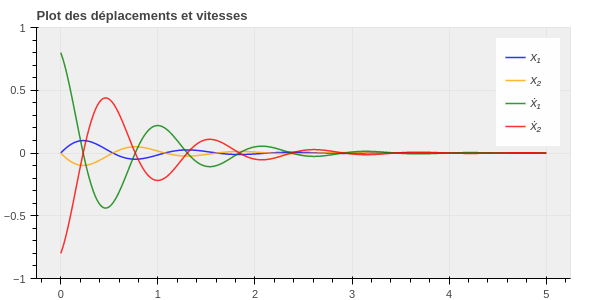
\includegraphics[width=\textwidth]{SimuDeplacement1D1.png}
        \caption{$v_0=v'_0 = 0.8$}
    \end{subfigure}
    \begin{subfigure}[t]{0.45\textwidth}
        \centering
        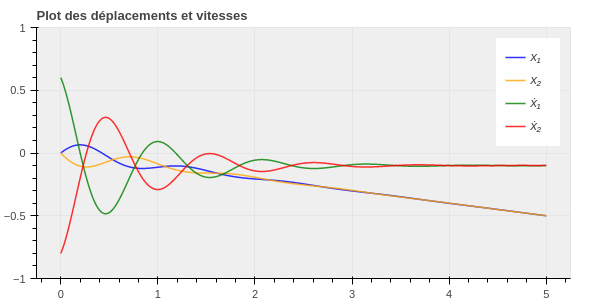
\includegraphics[width=\textwidth]{SimuDeplacement1D2.png}
        \caption{$v_0= 0.6$ et $v'_0 = 0.8$}
    \end{subfigure}

    \caption{Simulation du déplacement 1D d'un floe avec $m=1$, $k=18$, $\mu=1.3$, $t_{f}=5$. En règle générale, on observe le ralentissement du système et une convergence des déplacements vers l'état d'équilibre $Y_{eq}= (0,0,0,0)$ lorsque $v_0 = v'_0$.}
    \label{fig:simudept1d}
\end{figure*}

Avec $t_0= 0$, la solution analytique de ce système d'EDO du premier ordre à coefficients constants est unique et est donnée par.
\begin{align}
    Y(t) = \exp(tE)Y_0 \,.
\end{align}
Nous obtenons le théorème suivant:
\begin{theorem}[Convergence du modèle 1D isolé] \label{th:div1D}
    Les déplacements $x_1$ et $x_2$ des noeuds du floe 1D convergent si et seulement si leurs vitesses initiales sont des vecteurs opposés.
\end{theorem}

\begin{proof}

Le calcul des solution analytique est plus délicat. Il faudrait calculer l'exponentielle de la matrice $E$. Pour celà, nous devons diagonaliser (ou du moins trogonaliser) la matrice $E$. Son polynome caractéristique est donné par:
\begin{align*}    
\text{det}(E-\lambda I_4) &&&= \begin{vmatrix}
    -\lambda & 0 & 1 & 0 \\ 0 & -\lambda & 0& 1 \\ -\frac{k}{m} & \frac{k}{m} & -\frac{\mu}{m}-\lambda & \frac{\mu}{m} \\ \frac{k}{m} & -\frac{k}{m} & \frac{\mu}{m} & -\frac{\mu}{m} -\lambda
\end{vmatrix}, \\
    &&&= \frac{\lambda^2}{m} \left( m\lambda^2 + 2\mu\lambda + 2k \right).
\end{align*}
Posons $\Delta = 4\mu^2 - 8km$. On distingue deux cas:
\begin{itemize}
    \item Si $\Delta \geq 0$: on pose $\lambda_1 = \frac{-\mu - \sqrt{\mu^2 - 2km}}{m}$ et $\lambda_2 = \frac{-\mu + \sqrt{\mu^2 - 2km}}{m}$;
    \item Si $\Delta < 0$: on pose $\lambda_1 = \frac{-\mu - i\sqrt{2km - \mu^2}}{m}$ et $\lambda_2 = \frac{-\mu + i\sqrt{2km - \mu^2}}{m}$.
\end{itemize}
Nous avons donc exhiber les trois valeurs propres de notre matrice: $\lambda_0 = 0$, $\lambda_1$, et $\lambda_2$. Avec $\lambda$ désignant l'une des valeurs propres, on recherche les vecteurs $x = (x_1, x_2, x_3, x_4)^T \in \mathbb{R}^4$ appartenant aux sous espaces propres $E_\lambda$. On a:
\begin{align} \label{eq:espacepropre}
    Ex = \lambda x \Rightarrow \begin{dcases}
        x_3 = \lambda x_1 \\
        x_4 = \lambda x_2 \\
        -(k + \mu \lambda + m \lambda^2) x_1 + (k + \mu \lambda) x_2 = 0 \\
        (k + \mu \lambda) x_1 - (k + \mu \lambda + m \lambda^2) x_2 = 0
    \end{dcases}
\end{align}
\begin{itemize}
    \item Pour $\lambda = 0$, l'\cref{eq:espacepropre} revient à:
    \begin{align*}
        \begin{dcases}            
        x_3 = 0 \\
        x_4 = 0 \\
        x_1 - x_2 = 0
        \end{dcases}
    \end{align*} 
    On en déduit $E_0 = \text{vect}\{ e_1 \}$, avec $e_1 = (1,1,0,0)^T$.
    \item Pour $\lambda = \lambda_1, \lambda_2$, on remarque que $k + \mu \lambda + m \lambda^2 = - (k + \mu \lambda)$. l'\cref{eq:espacepropre} revient donc à:
    \begin{align*}
        \begin{dcases}            
        x_3 = \lambda x_1 \\
        x_4 = \lambda x_2 \\
        x_1 + x_2 = 0
        \end{dcases}
    \end{align*} 
    On en déduit donc $E_{\lambda_1} = \text{vect}\{ e_3 \}$, avec $e_3 = (1,-1,\lambda_1,-\lambda_1)^T$; et $E_{\lambda_2} = \text{vect}\{ e_4 \}$ avec $e_4 = (1,-1,\lambda_2,-\lambda_2)^T$.
\end{itemize}
La meutilisicté arithmetique de $\lambda = 0$ est differente de sa multiplicité géometrique. La matrice $E$ n'est donc pas diagonalisable. Son polynome caractéristique étant scindé, nous alons la trigonaliser. On pose donc une base $\mathcal{B}' = (v_1, v_2, v_3, v_4)$ dans laquelle la matrice $E$ s'exprime par:
\begin{align*}
    P^{-1}EP = \begin{pmatrix}
        0 & a & b & c \\ 0 & 0 & d & e \\ 0 & 0 & \lambda_1 & f \\ 0 & 0 & 0 & \lambda_2
    \end{pmatrix},
\end{align*}
où $P$ est la matrice de passage de la base canonique de $\mathbb{R}^4$ (notée $\mathcal{B}$) à $\mathcal{B}'$. On a:
\begin{itemize}
    \item Dans $\mathcal{B}'$, le vecteur $v_1$ s'écrit $v_1 = (1,0,0,0)^T$ et on a $P^{-1}EP v_1 = 0$. $v_1$ est donc le vecteur propre associé à $0$ et on prend $v_1 = e_1 = (1,1,0,0)^T$ dans $\mathcal{B}$;
    \item Dans $\mathcal{B}'$, le vecteur $v_2$ s'écrit $v_2 = (0,1,0,0)^T$ et on a $P^{-1}EP v_2 = a v_1$. On retourne dans $\mathcal{B}$ en posant $v_2 = (x_1, x_2, x_3, x_4)^T$ pour obtenir le système:
    \begin{align*}
        E v_2 = a v_1 \Rightarrow
        \begin{dcases}            
        x_3 = a  \\
        x_4 = a  \\
        x_1 - x_2 = 0
        \end{dcases}.
    \end{align*} 
    Avec $a = 1$, on écrit $v_2 = e_2 = (1,1,1,1)^T$.
    \item Dans $\mathcal{B}'$, le vecteur $v_3$ s'écrit $v_1 = (0,0,1,0)^T$ et on a $P^{-1}EP v_1 = \lambda_1 v_1 + bv_1 + d v_2$. En posant $b=d=0$, $v_1$ devient un vecteur propre associé à $\lambda_1$ et on prend $v_3 = e_3 = (1,-1,\lambda_1,-\lambda_1)^T$ dans $\mathcal{B}$;
    \item De facon similaire, on obtient $v_4 = e_4 = (1,-1,\lambda_2,-\lambda_2)^T$ en posant $c=e=f=0$.
\end{itemize}
Nous avons donc trigonaliser la matrice $E$, et on écrit :
\begin{align*}
    P^{-1}EP = A, \text{avec} A = \begin{pmatrix}
        0 & 1 & 0 & 0 \\ 0 & 0 & 0 & 0 \\ 0 & 0 & \lambda_1 & 0 \\ 0 & 0 & 0 & \lambda_2
    \end{pmatrix}, \text{  } P = \begin{pmatrix}
        1 & 1 & 1 & 1 \\ 1 & 1 & -1 & -1 \\ 0 & 1 & \lambda_1 & \lambda_2 \\ 0 & 1 & -\lambda_1 & -\lambda_2
    \end{pmatrix}, \text{ et } P^{-1} = \frac{1}{2}\begin{pmatrix}
        1 & 1 & -1 & -1 \\ 0 & 0 & 1 & 1 \\ \frac{\lambda_2}{\lambda_2-\lambda_1} & -\frac{\lambda_2}{\lambda_2-\lambda_1} & -\frac{1}{\lambda_2-\lambda_1} & \frac{1}{\lambda_2-\lambda_1} \\ -\frac{\lambda_1}{\lambda_2-\lambda_1} & \frac{\lambda_1}{\lambda_2-\lambda_1} & \frac{1}{\lambda_2-\lambda_1} & -\frac{1}{\lambda_2-\lambda_1}
    \end{pmatrix}.
\end{align*}
La matrice $A$ se décompose en somme d'une matrice diagonale et d'une matrice nilpotente $A = D+N$ avec:
\begin{align*}
    D = \begin{pmatrix}
        0 & 0 & 0 & 0 \\ 0 & 0 & 0 & 0 \\ 0 & 0 & \lambda_1 & 0 \\ 0 & 0 & 0 & \lambda_2
    \end{pmatrix}, \text{ et } N = \begin{pmatrix}
        0 & 1 & 0 & 0 \\ 0 & 0 & 0 & 0 \\ 0 & 0 & 0 & 0 \\ 0 & 0 & 0 & 0
    \end{pmatrix}.
\end{align*}
En posant $E = P(D+N)P^{-1}$, nous pouvons facilemtn calculer $\forall t \in \mathbb{R}$, $\exp(tE) = P\exp(tD)\exp(tN)P^{-1}$. Ce calcul délicat donne (à l'aide du logiciel de calcul symbolique $\verb|Symbolab|$):
\begin{align*}
    \exp(tE) = \tiny \frac{1}{2(\lambda_2 - \lambda_1)}\begin{pmatrix} 
        \lambda_2e^{t\lambda_1} + \lambda_2 - \lambda_1 - \lambda_1e^{t\lambda_2} & -\lambda_2e^{t\lambda_1} + \lambda_2 - \lambda_1 + \lambda_1e^{t\lambda_2} & t(\lambda_2 -\lambda_1) - e^{t\lambda_1} + e^{t\lambda_2} & t(\lambda_2 -\lambda_1) + e^{t\lambda_1} - e^{t\lambda_2} \\
         -\lambda_2e^{t\lambda_1} + \lambda_2 - \lambda_1 + \lambda_1e^{t\lambda_2} & \lambda_2e^{t\lambda_1} + \lambda_2 - \lambda_1 - \lambda_1e^{t\lambda_2} & t(\lambda_2 -\lambda_1) + e^{t\lambda_1} - e^{t\lambda_2} & t(\lambda_2 -\lambda_1) - e^{t\lambda_1} + e^{t\lambda_2} \\
          \lambda_1\lambda_2 (e^{t\lambda_1} - e^{t\lambda_2}) & \lambda_1\lambda_2 (e^{t\lambda_2} - e^{t\lambda_1})  & -\lambda_1e^{t\lambda_1} + \lambda_2 - \lambda_1 + \lambda_2e^{t\lambda_2} & \lambda_1e^{t\lambda_1} + \lambda_2 - \lambda_1 - \lambda_2e^{t\lambda_2} \\
          \lambda_1\lambda_2 (e^{t\lambda_2} - e^{t\lambda_1})  & \lambda_1\lambda_2 (e^{t\lambda_1} - e^{t\lambda_2})  & \lambda_1e^{t\lambda_1} + \lambda_2 - \lambda_1 - \lambda_2e^{t\lambda_2} & -\lambda_1e^{t\lambda_1} + \lambda_2 - \lambda_1 + \lambda_2e^{t\lambda_2}
    \end{pmatrix}.
\end{align*}
Rappelons nous que la solution du problème de Cauchy \cref{eq:dep1d} est donnée par $Y(t) = \exp(tE)Y_0$, avec $Y_0 = (0,0,v_0,-v'_0)$. Le calcul du déplacement $x_1$ donne:
\begin{align} \label{eq:solreel}
    x_1(t) = \frac{t}{2}\left( v_0 - v'_0 \right) \textcolor{red}{+} \frac{e^{t\lambda_1} - e^{t\lambda_2}}{2(\lambda_2 - \lambda_1)}\left( v_0 + v'_0 \right).
\end{align}
Le cas où $\Delta < 0$ (à étudier dans $\mathbb{C}$) peut se ramener au cas réel (dans $\mathbb{R}$) en posant $\lambda_1 = \alpha + i \beta$ et $\lambda_2 = \alpha - i \beta = \bar{\lambda}_1$ (avec $\alpha = -\frac{\mu}{m}$ et $\beta = -\frac{\sqrt{2km - \mu^2}}{m}$). En remarquant que $\sin(\beta t) = \frac{e^{i\beta t} - e^{-i\beta t}}{2i}$, on obtient:
\begin{align} \label{eq:solcomplexe}
    x_1(t) = \frac{t}{2}\left( v_0 - v'_0 \right) \textcolor{red}{+} \frac{e^{\alpha t} \sin(\beta t)}{2\beta} \left( v_0 + v'_0 \right).
\end{align}
Les \cref{eq:solreel,eq:solcomplexe} permettent d'observer que le déplacement $x_1$ ne converge pas lorsque $t \rightarrow +\infty$, à moins que $v_0 = v'_0$, ce qui est observé à la \cref{fig:simudept1d}. On tire les mêmes conclusions pour $x_2$ en effectuant un raisonnement similaire.

\end{proof}








\subsubsection{Collision parfaitement inélastique avec un floe encastré à l'instant initial}

Nous effectuons ici une modélisation 1D de notre problème. Un floe est modélisé par un système masse-ressort de deux nœuds. Le floe 1 est immobilisé face au mur, et le floe 2 approche à la vitesse $\bvec{v}_0$. On identifie les nœuds $q_0$ et $p_0$ de la section précédente à leur masses respectives $m$ et $m'$ (voir \cref{fig:contact1d}).
\begin{figure}[!h]
    \centering
    \frame{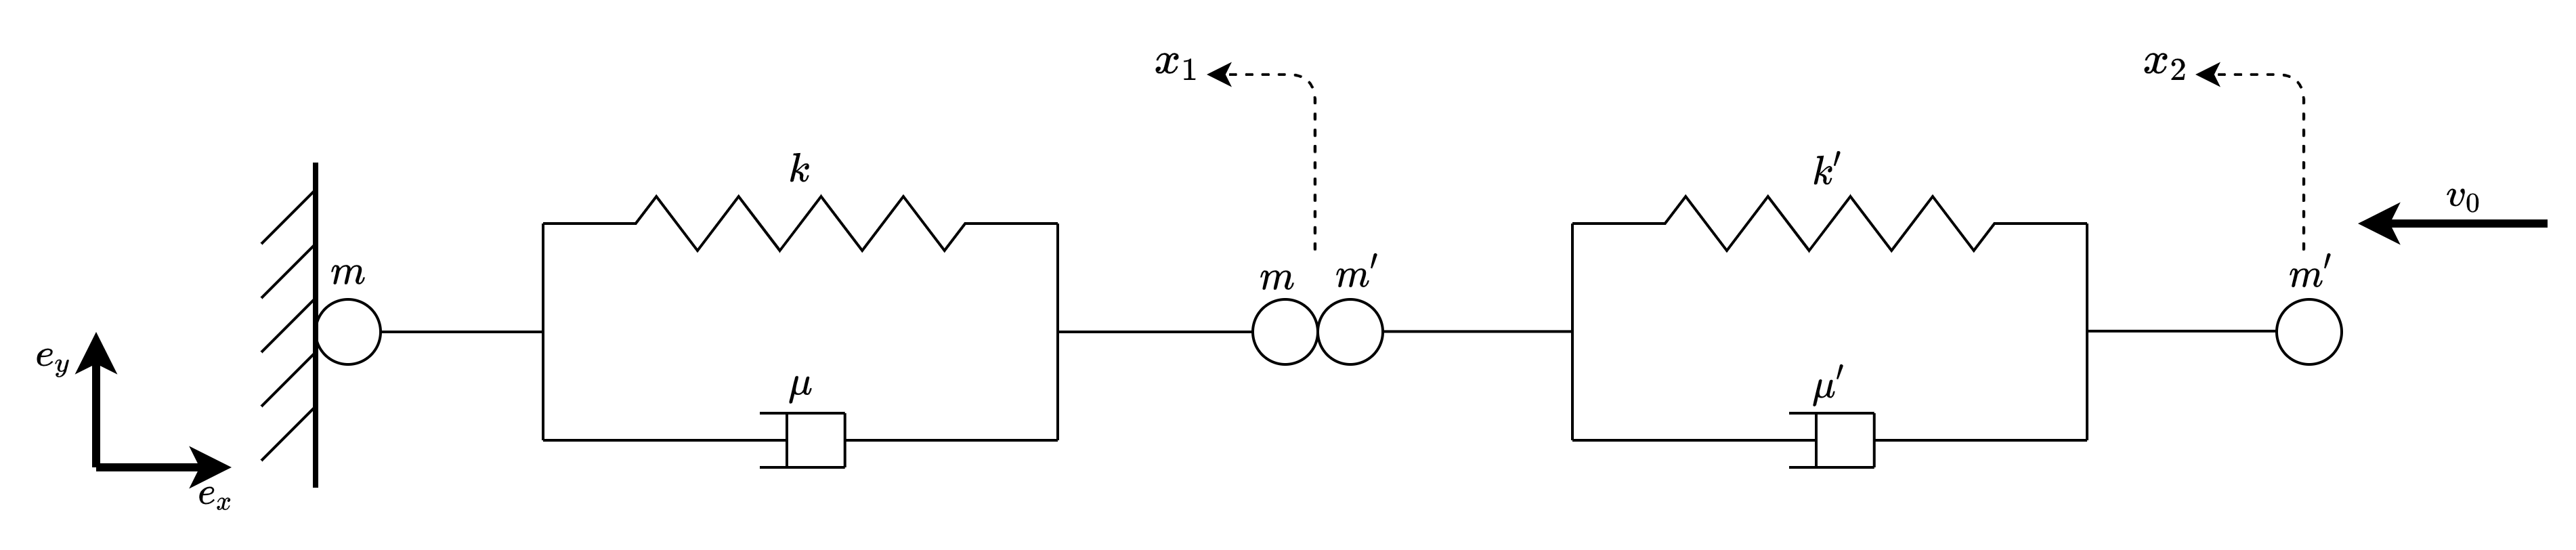
\includegraphics[width=0.8\textwidth]{Percussion1D-Systeme}}
    \caption{Contact 1D parfaitement inélastique entre deux floes. Le floe percuté étant immobile et coincé au mur avant le choc.}
    \label{fig:contact1d}
\end{figure}

\noindent On suppose que durant la dynamique non régulière, les masses $m$ et $m'$ en contact forment une seule masse\footnote{Cette simplification a pour principal avantage de supprimer le traitement de la force de contact entre les deux masses.}
$m+m'$ dont
le déplacement est donné par la variable $x_1(t)$. Le déplacement de la masse $m'$ à l'autre bout du floe percuteur est nommé
$x_2(t)$. La masse $m$ qui est fixée au mur ne sera pas étudiée ici. Nous faisons à présent le bilan des forces qui
s'exercent ces
deux masses.
\begin{figure}[!h]
     \begin{subfigure}[b]{0.4\textwidth}
         \centering
         \frame{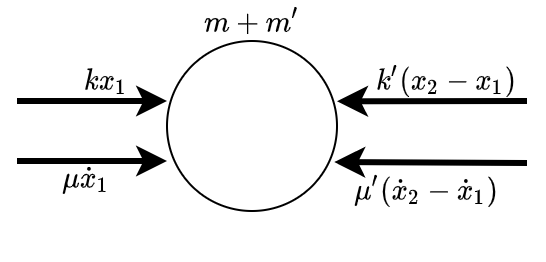
\includegraphics[width=\textwidth]{Percussion1D-Masse1}}
         \caption{Sur $m+m'$.}
         \label{fig:bilan11}
     \end{subfigure}
%     \hfill
     \begin{subfigure}[b]{0.3\textwidth}
         \centering
         \frame{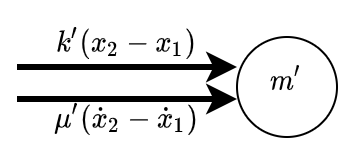
\includegraphics[width=\textwidth]{Percussion1D-Masse2}}
         \caption{Sur $m'$.}
         \label{fig:bilan12}
     \end{subfigure}
        \caption{Bilan des forces appliquée sur les noeuds du système. Les valeurs indiquées sont les intensitées
            (positives) des forces durant une phase imaginée de compression des ressorts ($\bvec{v}_0 <0$ et donc
            $x_1 <0$). Pour obtenir l'intesité de la force de rappel du ressort $k'$, on peut imaginer $x_1$ imobile
            (on aura $x_2 < 0$, d'où $x_1 - x_2 > 0$) (voir \parencite{homodeling}).}
        \label{fig:bilan}
\end{figure}

\noindent En orientant convenablement le système (voir \cref{fig:contact1d}), on applique la loi de Newton-Euler linéaire
pour obtenir le système suivant et ses conditions initiales \footnote{J'ai des doutes sur cette condition
initiale. La vitesse initiale de $x_1$ est-elle vraiment nulle?}:
\begin{align}
    \begin{dcases}
    (m+m')\ddot x_1 = -kx_1 - \mu \dot x_1 + k'(x_2 - x_1) + \mu'(\dot x_2 - \dot x_1) \\
        m' \ddot x_2 =  -k'(x_2 - x_1) - \mu'(\dot x_2 - \dot x_1) 
    \end{dcases}
\end{align}
À l'instant initial $t_0$, on a le système suivant
\begin{align} \label{eq:percussion1d}
    \begin{dcases}
    (x_1(t_0), x_2(t_0)) = (0,0) \\
    (\dot x_1(t_0), \dot x_2(t_0)) = (0,-v_0)
    \end{dcases}
\end{align}
En posant $X = (x_1, x_2)^T \in \mathbb{R}^2$, l' \cref{eq:percussion1d} devient
\begin{align}
    \underbrace{\mymat{m+m'}{0}{0}{m'}}_{A} \myvec{\ddot{x}_1}{\ddot{x}_2} = \underbrace{\mymat{-\mu -
    \mu^\prime}{\mu'}{\mu'}{-\mu'}}_{B}
    \myvec{\dot{x}_1}{\dot{x}_2} + \underbrace{\mymat{-k-k'}{k'}{k'}{-k'}}_{C} \myvec{x_1}{x_2} \,.
\end{align}
Puisque $m, m'\neq 0$, la matrice $A$ est inversible et on obtient au final le problème de Cauchy suivant:
\begin{align} \label{eq:percussion1d2}
    \begin{dcases}
        \ddot{X}(t) = B' \dot{X}(t) + C'X(t) \,, \\
        (X(t_0), \dot X (t_0)) = \left( \myvec{0}{0}, \myvec{0}{-v_0} \right) \,,
    \end{dcases}
\end{align}
avec $B' = A^{-1}B$ et $C' = A^{-1}C$.

\noindent Il s'agit la d'un système d'EDO du deuxième ordre à coefficients constants. Transformons le en un système du premier ordre pour
une résolution plus aisée. On pose donc $Y= (X, \dot X)^T = (x_1, x_2, \dot{x}_1, \dot{x}_2)^T \in \mathbb{R}^4$ et le
système
\ref{eq:percussion1d2}
devient
\begin{align} \label{eq:systeme1d}
    \begin{dcases}
        \dot{Y}(t)= E Y(t) \\
        Y_0 = Y(t_0) = (0,0,0,-v_0)^T
    \end{dcases}
\end{align}
avec la matrice par blocs \[ E = \mymat{0}{I_2}{C'}{B'} \,, \] où $I_2$ désigne la matrice identité de
$\mathbb{R}^{2\times2}$.

\noindent Avec $t_0= 0$, la solution de ce système d'EDO du premier ordre à coefficients constants est unique et est donnée par
\begin{align}
    Y(t) = \exp(tE)Y_0
\end{align}

La résolution analytique du système passe par le calcul de l'exponentielle de la matrice $E \in \mathbb{R}^4$, ce qui s'avère difficile du à la taille de ladite matrice. Nous optons donc pour une solution numérique (voir figure \cref{fig:simucontact1d} issue du notebook $\verb|code/simu1D/Percussion1D-1.ipynb|$ ) \ldots
\begin{figure}[!h]
    \centering
    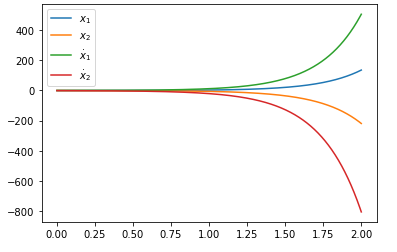
\includegraphics[width=0.4\textwidth]{SimuPercussion1D.png}
    \caption{Simulation de la percussion 1D entre deux floes avec $m=1$, $m'=1$, $k=16$, $k'=5$, $\mu=6$,
        $\mu'=2$, $v_0=-1.0$, $t_{f}=32$. On observe effectivement le ralentissement du système et une convergence
        vers l'état d'équilibre $Y_{eq}= (0,0,0,0)$.}
    \label{fig:simucontact1d}
\end{figure}

\noindent Pour certaines valeurs (specifiquement de $\mu$ et $\mu'$), on constate que le système converge vers son état d'équilibre attendu $Y_{eq} = (0,0,0,0)$. Il nous reste dans cette section:
\begin{enumerate}
    \item Calculer analytiquement et numériquement tous les état d'équilibres $Y_{eq} \in \ker(E)$; distinguer les états stables des autres.
    \item Calculer analytiquement l'exponentielle de la matrice $E$, et donner l'expression de la solution; déduire la condition sur les parametres pour que le système converge vers l'état d'équilibre voulu.
\end{enumerate} 







\subsubsection{Collision parfaitement inélastique sans présence du mur}

Contrairement au cas étudié dans la section précédente, le mur est supprimé dans cette section. On obtient donc une troisième variable $x_3$ décrivant le comportement du noeud qui était rattaché au mur. La schéma régissant ce système est donnée à la \cref{fig:contact1d2}. Le bilan des forces appliquées aux noeuds est présenté à la \cref{fig:bilan2}.

\begin{figure}[!h]
    \centering
    \frame{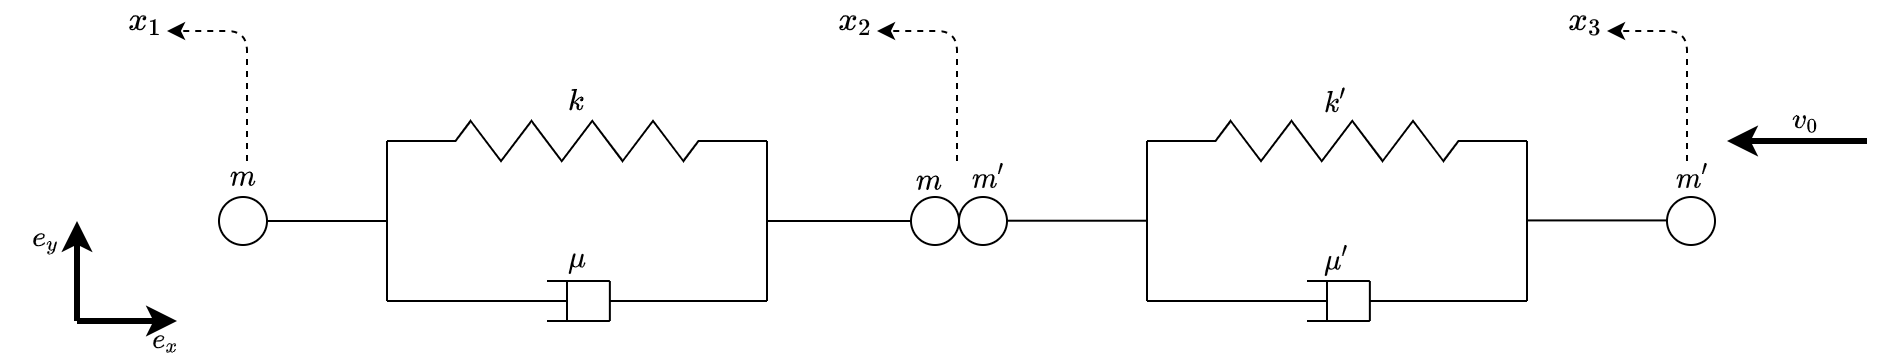
\includegraphics[width=0.8\textwidth]{Percussion1D-Systeme-2}}
    \caption{Contact 1D parfaitement inélastique entre deux floes. Le floe percuté étant non immobile (et non coincé au mur) avant le choc. On représnte également les variables $x_1$, $x_2$, et $x_3$ décrivant les movements de chaque noeud.}
    \label{fig:contact1d2}
\end{figure}

\begin{figure}[!h]
    \begin{subfigure}[b]{0.25\textwidth}
        \centering
        \frame{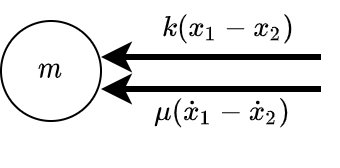
\includegraphics[width=\textwidth]{Percussion1D2-Masse1.png}}
        \caption{Sur $m$.}
        \label{fig:bilan12}
    \end{subfigure}
%     \hfill
    \begin{subfigure}[b]{0.31\textwidth}
        \centering
        \frame{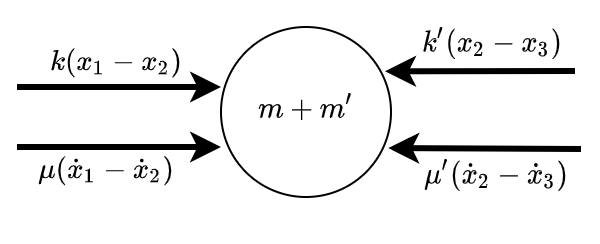
\includegraphics[width=\textwidth]{Percussion1D2-Masse2}}
        \caption{Sur $m+m'$.}
        \label{fig:bilan22}
    \end{subfigure}
%     \hfill
    \begin{subfigure}[b]{0.23\textwidth}
        \centering
        \frame{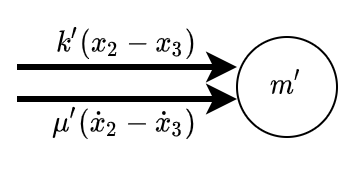
\includegraphics[width=\textwidth]{Percussion1D2-Masse3}}
        \caption{Sur $m'$.}
        \label{fig:bilan32}
    \end{subfigure}
       \caption{Bilan des forces appliquée sur les noeuds du système. On procède de facon similaire à \cref{fig:bilan} pour obtenir les sens et les intensités de ces forces.}
       \label{fig:bilan2}
\end{figure}

\noindent Comme précédement, nous appliqons les lois de Newton pour obtenir:
\begin{align}
    \begin{dcases}
    m\ddot x_1 = -k(x_1 - x_2) - \mu (\dot x_1 - \dot x_2) \,, \\
    (m+m')\ddot x_2 = k(x_1 - x_2) + \mu (\dot x_1 - \dot x_2) - k'(x_2 - x_3) - \mu'(\dot x_2 - \dot x_3) \,, \\
        m' \ddot x_3 =  k'(x_2 - x_3) + \mu'(\dot x_2 - \dot x_3) \,. 
    \end{dcases}
\end{align}
Sous forme matricielle, on a
\begin{align}
    \underbrace{\mybigmat{m}{0}{0}{0}{m+m'}{0}{0}{0}{m'}}_{A} \mybigvec{\ddot{x}_1}{\ddot{x}_2}{\ddot{x}_3} =  
    \underbrace{\mybigmat{-k}{k}{0}{k}{-k-k'}{k}{0}{k'}{-k'}}_{B} \mybigvec{x_1}{x_2}{x_3} + 
    \underbrace{\mybigmat{-\mu}{\mu}{0}{\mu}{-\mu-\mu'}{\mu'}{0}{\mu'}{-\mu'}}_{C} \mybigvec{\dot{x}_1}{\dot{x}_2}{\dot{x}_3} \,.
\end{align}
Puisque $m, m'\neq 0$, la matrice $A$ est inversible. En posant $X = (x_1, x_2, x_3)^T \in \mathbb{R}^3$, le système d'EDO revient à l' \cref{eq:percussion1d22} suivante:
\begin{align} \label{eq:percussion1d22}
        \ddot{X}(t) = B' X(t) + C'\dot{X}(t) \,, 
\end{align}
où $B' = A^{-1}B$ et $C' = A^{-1}C$. On pose ensuite $Y= (X, \dot X)^T \in \mathbb{R}^6$ et le système \cref{eq:percussion1d22} devient 
\begin{align} \label{eq:systeme1d2}
        \dot{Y}(t)= E Y(t)
\end{align}
avec $$ E = \mymat{0}{I_3}{B'}{C'} \,.$$


Remarquons qu'en enlevant le mur à gauche du domaine (voir \cref{fig:contact1d}), le système est devenu isolé. Nous pouvons donc appliquer la conservation de la quantité de mouvement pour identifier la vitesse de l'ensemble $m+m'$ après collision et fixation de la masse $m'$ (à vitesse $\bvec{v}_0$) sur la masse $m$ (de vitesse $\bvec{v}'_0$)\footnote{Le vecteur $\bvec{v}'_0$ n'est pas marqué à la \cref{fig:contact1d2} (i.e. $\bvec{v}'_0 = 0$). L'introduction de ce vecteur permet de généraliser le problème.}. Pour simplifier les calculs, nous considérons les floes comme des solides rigides. La vitesse de l'ensemble juste après collision est notée $v_f$, et les quantités de mouvement avant et après choc sont notées $P_{\text{avant}}$ et $P_{\text{après}}$. On a :
\begin{align*}
    & \quad P_{\text{avant}} = P_{\text{après}} \\
    \Rightarrow & \quad 2m \bvec{v}_0 + 2m'\bvec{v'}_0 = (2m + 2m') \bvec{v}_f \\
    \Rightarrow & \quad \bvec{v}_f = \frac{m \bvec{v}_0 + m'\bvec{v'}_0}{m+m'}
\end{align*} 

\noindent On introduit ces conditions initiales dans l'\cref{eq:systeme1d2} pour obtenir le système de Cauchy ci-bas. Le résulat de la simulation est présenté à la figure \cref{fig:simucontact1d2} (issue du notebook $\verb|code/simu1D/Percussion1D-2.ipynb|$). 
\begin{align} \label{eq:systeme1d3}
    \begin{dcases}
        \dot{Y}(t)= E Y(t) \,, \\
        Y(t_0) = Y_0 = -v_f(0,0,0,1,1,1) \,.        
    \end{dcases}
\end{align}

\begin{figure}[!h]
    \centering
    \begin{subfigure}{0.45\textwidth}
        \centering
        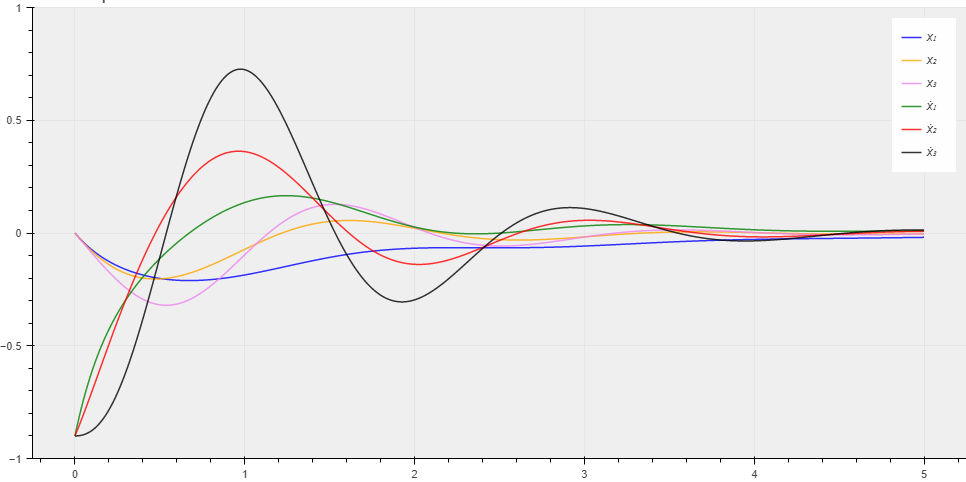
\includegraphics[width=\textwidth]{SimuPercussion1D2.png}
        \caption{$k=3$}
    \end{subfigure}
    \begin{subfigure}{0.45\textwidth}
        \centering
        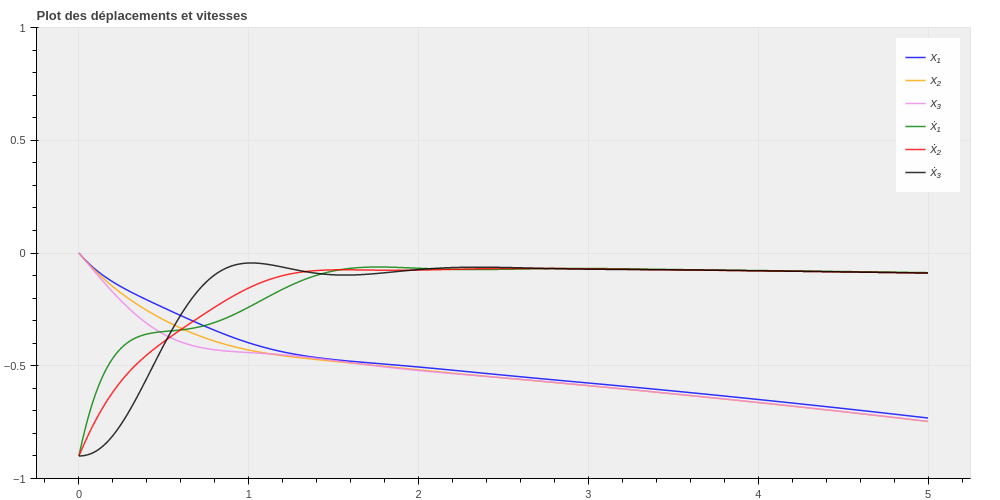
\includegraphics[width=\textwidth]{SimuPercussion1D2NonConv.png}
        \caption{$k=23$}
    \end{subfigure}

    \caption{Simulation de la percussion 1D entre deux floes (sans présence du mur) avec $m=1$, $m'=1$, $k'=22$, $\mu=6$, $\mu'=2$, $v_0=-1.8$, $t_{f}=5$. Sous certaines conditions (forte dissipation, raideur du floe percuté élevée, etc.), on observe le ralentissement du système et une convergence vers l'état d'équilibre $Y_{eq}=(0,0,0,0,0,0)$.} 
    \label{fig:simucontact1d2}
\end{figure}

\noindent La \cref{fig:simucontact1d2} permet d'observer la nuance avec le problème de contact parfaitemetn inélastique. Il est difficile de distinguer les cas qui aboutissent à une convergences des déplacements de ceux qui divergent. Observons donc à présent un problème de contact inélastique avec séparation des masses.




\subsubsection{Collision inélastique avec séparation des masses}

Reprennons le cas du contact 1D et étudions ce qui se passe durant l'intervale de temps $\tdelta = [\tmoins, \tplus]$ de la collision. Cette fois, pour étudier la dynamique non régulière, nous décidons de séparer les masses $m$ et $m'$ en contact (et ce même durant le contact). Le système résultant est très similaire aux deux cas traités précédemment (\cref{fig:contact1d,fig:contact1d2}), et nous le présentons à la \cref{fig:contact1d3} ci-bas, et son bilan de forces à la \cref{fig:bilan3}.

\begin{figure}[!h]
    \centering
    \frame{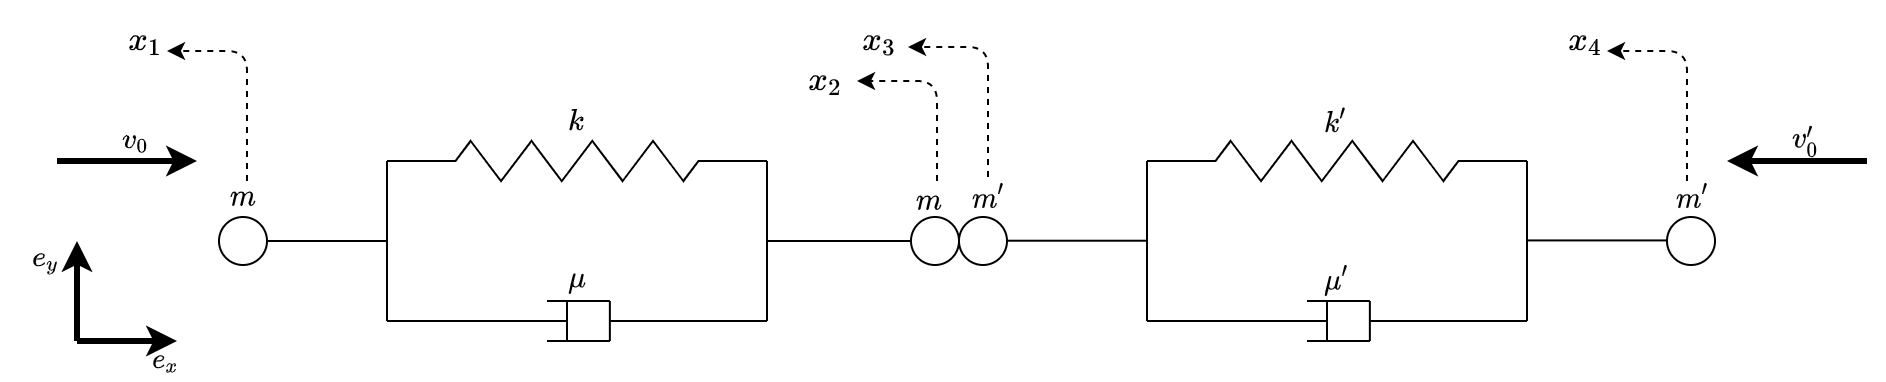
\includegraphics[width=0.8\textwidth]{Percussion1D-Systeme-3}}
    \caption{Contact 1D inélastique entre deux floes. Durant le choc, les nœuds $m$ et $m'$ en contact sont étudiés séparement. On représnte les variables $x_1$, $x_2$, $x_3$, et $x_4$ décrivant les movements de chaque noeud.}
    \label{fig:contact1d3}
\end{figure}


\begin{figure}[!h]
    \begin{subfigure}[b]{0.30\textwidth}
        \centering
        \frame{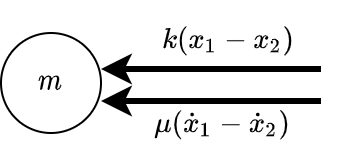
\includegraphics[width=\textwidth]{Percussion1D3-Masse1.png}}
        \caption{Sur $m$ de gauche ($x_1$).}
        \label{fig:bilan13}
    \end{subfigure}
%     \hfill
    \begin{subfigure}[b]{0.35\textwidth}
        \centering
        \frame{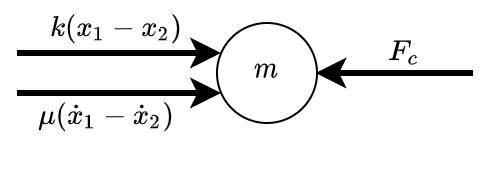
\includegraphics[width=\textwidth]{Percussion1D3-Masse2}}
        \caption{Sur $m$ de droite ($x_2$).}
        \label{fig:bilan23}
    \end{subfigure}
%     \hfill
    \begin{subfigure}[b]{0.35\textwidth}
        \centering
        \frame{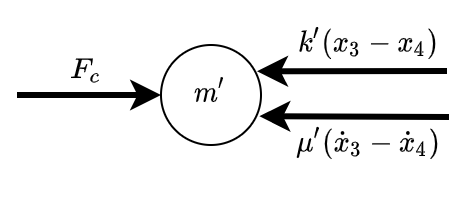
\includegraphics[width=\textwidth]{Percussion1D3-Masse3}}
        \caption{Sur $m'$ de gauche ($x_3$).}
        \label{fig:bilan33}
    \end{subfigure}
%     \hfill
    \begin{subfigure}[b]{0.30\textwidth}
        \centering
        \frame{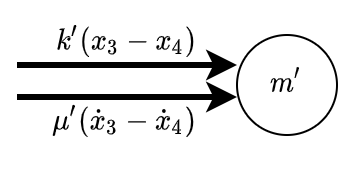
\includegraphics[width=\textwidth]{Percussion1D3-Masse4}}
        \caption{Sur $m'$ de droite ($x_4$).}
        \label{fig:bilan43}
    \end{subfigure}
       \caption{Bilan des forces appliquée sur les $4$ noeuds du système. On procède de facon similaire aux \cref{fig:bilan,fig:bilan2} pour obtenir les sens et les intensités de ces forces. $F_c$ représente la force de contact dont l'intensité est inconnue.}
       \label{fig:bilan3}
\end{figure}

\noindent Comme précédement, nous appliqons les lois de Newton pour obtenir:
\begin{align}
    \begin{dcases}
    m\ddot x_1 = -k(x_1 - x_2) - \mu (\dot x_1 - \dot x_2) \,, \\
    m\ddot x_2 = k(x_1 - x_2) + \mu (\dot x_1 - \dot x_2) - F_c \,, \\
    m'\ddot x_3 = - k'(x_3 - x_4) - \mu'(\dot x_3 - \dot x_4) + F_c \,, \\
        m' \ddot x_4 =  k'(x_3 - x_4) + \mu'(\dot x_3 - \dot x_4) \,. 
    \end{dcases}
\end{align}
On additionne membre à membre les équations régissant les mouvements de $x_2$ et $x_3$ pour éliminer la force de contact $F_c$ et obtenir le système:
% \begin{align}\label{eq:systeme3test}
    \begin{subnumcases}{}
    m\ddot x_1 = -k(x_1 - x_2) - \mu (\dot x_1 - \dot x_2) \,, \label{eq:sys1D1}\\
    m\ddot x_2 + m'\ddot x_3 = k(x_1 - x_2) + \mu (\dot x_1 - \dot x_2) - k'(x_3 - x_4) - \mu'(\dot x_3 - \dot x_4) \,, \label{eq:sys1D2} \\
        m' \ddot x_4 =  k'(x_3 - x_4) + \mu'(\dot x_3 - \dot x_4) \,. \label{eq:sys1D3}
    \end{subnumcases}
% \end{align}
Remarquons que ce système reviens au même systeme étudié dans la partie précédente en posant $x_2(t) = x_3(t) $ p.p. En effet, durant la phase de contact, les massess $m$ et $m'$ peuvent etrs étudiées comme une unique masse $m+m'$. La grosse diffculté qui ressort de cette modélisation est la définitions de la vitesse initiale de l'ensemble $m+m'$. Celà dit, nous cherchons à trouver les vitessses $\dot x_1(\tplus)$, $\dot x_2(\tplus)$, $\dot x_3(\tplus)$ et $\dot x_4(\tplus)$ immédiatemetn après la collision. De par la ressemblance de ce modèle avec celui de la section précédente (voir \cref{eq:systeme1d2}), nous réutilisons les quantités $\dot x_1$ et $\dot x_4$ données par ce système (l'\cref{eq:systeme1d2} dans lequel $x_2$ et $x_3$ sont confondus). On peut se permertre une telle approximation car $x_1$ et $x_4$ n'interviennent pas directemetn dans la collision. De plus, la quantité $k(x_1 - x_2) + \mu (\dot x_1 - \dot x_2) - k'(x_3 - x_4) - \mu'(\dot x_3 - \dot x_4)$
% \begin{align}
%     I = k(x_1 - x_2) + \mu (\dot x_1 - \dot x_2) - k'(x_3 - x_4) - \mu'(\dot x_3 - \dot x_4)    
% \end{align}
est aussi calculé suivant le modèle \cref{eq:systeme1d2} (voir l'article \parencite{tommasino2020effect} pour une modélisation similaire). Il ne nous reste véritablement que $2$ inconnue dans notre dynamique irrégulière.

\noindent Intégrons l'équation (\ref{eq:sys1D2}) entre les instants $\tmoins$ et $\tplus$. On obtient:
\begin{align}    \label{eq:debuteq1}
    \int_{\tmoins}^{\tplus} m\ddot x_2 + m'\ddot x_3 \diff t = \underbrace{\int_{\tmoins}^{\tplus} k(x_1 - x_2) + \mu (\dot x_1 - \dot x_2) - k'(x_3 - x_4) - \mu'(\dot x_3 - \dot x_4) \diff t}_{I} \,.
\end{align}
Afin d'éviter toute confusion, nous notons $v_0 = \dot{x}_2(\tmoins)$ et $v'_0 = \dot{x}_3(\tmoins)$ les vitesses des noeuds en contact avant collision, et $V_0 = \dot{x}_2(\tplus)$ et $V'_0 = \dot{x}_3(\tplus)$ les vitesses après contact. L'équation \cref{eq:debuteq1} devient donc:
\begin{align} \label{eq:crammer1}
    mV_0 + m'V'_0 = I + mv_0 + m'v'_0 \,.
\end{align}
À présent, nous pouvons étudier l'énergie cinétique du système à travers le coefficient de restitution $\varepsilon$ \footnote{Le coefficient de restitution est le même que celui utilisé dans la thèse \parencite{rabatel2015thesis}.}. On suppose (algébriquement) que les noeuds prennent des directions indiquées à la \cref{fig:contact1dapres}. 
\begin{figure}[!h]
    \centering
    \frame{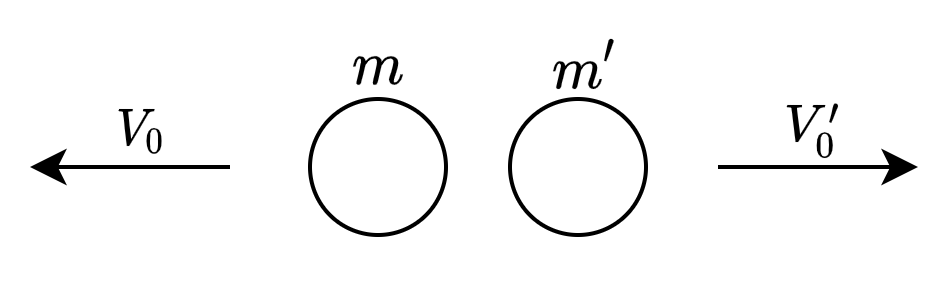
\includegraphics[width=0.6\textwidth]{Percussion1D3-Apres.png}}
    \caption{Situation après contact 1D.}
    \label{fig:contact1dapres}
\end{figure}

\noindent On obtient l'\cref{eq:crammer2}:
\begin{align} \label{eq:crammer2}
    - V_0 + V'_0 = \varepsilon (v_0 - v'_0) \,.
\end{align}
Le système de Cramer qui découle des \cref{eq:crammer1,eq:crammer2} permet d'obtenir les expressions:
\begin{align}
    V_0 = \frac{I + (m+\varepsilon m')v_0 + (1-\varepsilon)m'v'_0}{m+m'} \,, \quad V'_0 = \frac{I + (1-\varepsilon)mv_0 + (m'+\varepsilon m)v'_0}{m+m'}\,.
\end{align}

Nous faisons donc ici la grosse hypothèse que \underline{le mouvement de $x_2$ et $x_3$ devient uniforme après la collision}. Une fois leur vitesses "initiales"\footnote{Ces vitesses sont les vitesses de départ pour le deuxième phase de la percussion.} obtenues, on calcule donc les déplacements des différents noeuds des réseaux, et les fractures éventuelles qui s'en suivent. 

\paragraph{Analyse du modèle.} Observons le premier floe de plus près:
\begin{itemize}
    \item Son noeud de gauche $x_1$ a pour vitesse $v_0$ avant et le choc et conserve cette vitesse après le choc;
    \item Son noeud de droite $x_2$ a pour vitesse $v_0$ avant le choc, mais passe de facon discontinue à $V_0$ apres le choc.
\end{itemize}
N'ayant aucune garantie que les vecteurs vitesses $v_0$ et $V_0$ seront opposés immédiatemetn après le choc, nous ne pouvons garantir la convergence de ce modèle (voir \cref{th:div1D}). Ce modèle dégénère (probablement) après la première collision. Effectuons à présent une modélisation 2D et observons si le même problème se repète.

%%-------Pas vrai
% Pour $\varepsilon \neq 0$, l'\cref{eq:crammer2} permet de constater que $V_0 = V'_0$ si et seulement si $v_0 = v'_0$. En se basant sur le \cref{th:div1D}, nous pouvons donc énoncer le corrolaire suivant:

% \begin{corollary} \label{cr:div1D}
%     Le modèle de collision inélastique 1D avec séparation des masses converge si les vitesses des noeuds avant le choc sont des vecteurs opposés.

%     Le modèle de collision inélastique 1D avec séparation des masses converge si et seulement si leurs vitesses initiales sont des vecteurs opposés.
% \end{corollary}
% \begin{proof}
%     La preuve découle immédiatement du \cref{th:div1D}.
% \end{proof}

% \noindent Le \cref{cr:div1D} permet de constater les limites de notre modélisation 1D. En effet, les moceaux de glace dans la MIZ ne dérivent pas tous à la meme vitesse. Effectuons à présent une modélisation 2D et observons si le même problème se repète.




\subsection{Modélisation et simulation 2D}









\subsubsection{Déplacement d'un floe isolé}

Étudions le comportement d'un floe de glace 2D modélisé par un réseau de ressorts (3 ressort, 3 dispositif viseux, et 3 noeuds) (voir \cref{fig:deplacement2d}).
\begin{figure}[!h]
    \centering
    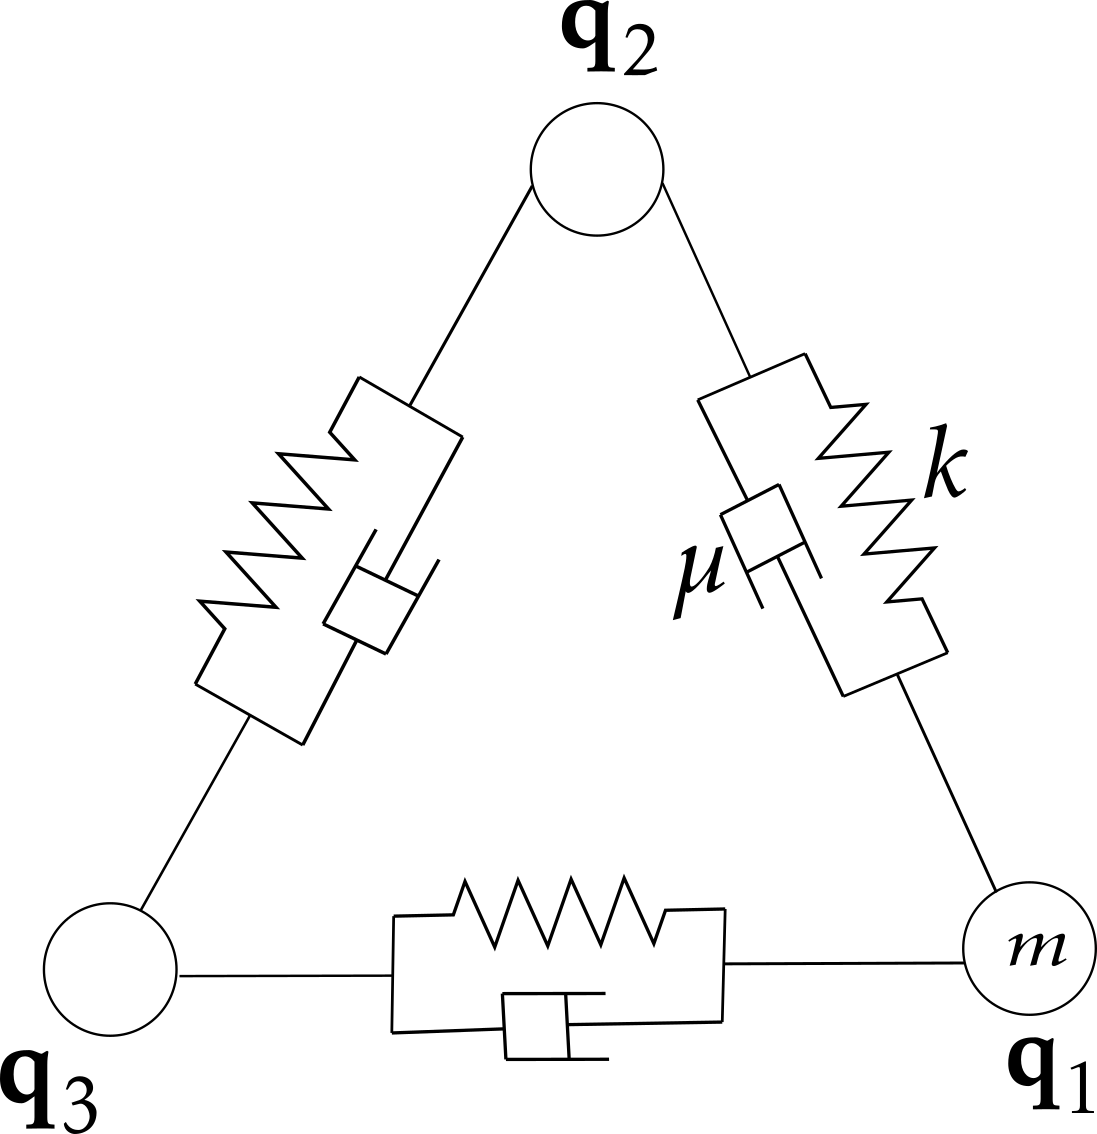
\includegraphics[width=0.3\textwidth]{Deplacement2D-1.png}
    \caption{Floe de glace 2D modélisé par un réseau de ressorts. Le floe est isolé de toutes forces extérieurs. Tous les neouds du réseau ont la même masse $m$, tous les ressorts on la même raideur $k$, et tous les dispositifs visquens ont le même coefficient $\mu$.}
    \label{fig:deplacement2d}
\end{figure}


\noindent Comme nous l'avons présenté aux \cref{eq:F0,eq:e}, le système de la \cref{fig:deplacement2d} est régit par l' équation:
\begin{align} \label{eq:eprime2}
    \forall i \in \mathbb{Z}/3\mathbb{Z}, \quad m \ddot{\bvec{q}}_i = \sum_{j=i+1}^{i+2}C_{ij} \left[  k \left( \Vert \bvec{q}_j - \bvec{q}_i \Vert - L_{ij} \right) \bvec{u}_{ij} - \mu \left\langle \bvec{\dot{q}}_j - \bvec{\dot{q}}_i, \, \bvec{u}_{ij}  \right\rangle  \bvec{u}_{ij}  \right]  , 
\end{align}
où $L_{ij}$ représente la longeur au repos du ressort entre les noeuds $i$ et $j$, et $C_{ij}$ indique si les noeuds $i$ et $j$ sont connectés ou non (pour ce modèle 2D simple, $C_{ij} = 1 \, \forall 0 \leq i,j \leq 2$). Le vecteur unitaire $\bvec{u}_{ij}$ vaut:
$$
\bvec{u}_{ij} = \frac{\bvec{q}_j - \bvec{q}_i}{\Vert \bvec{q}_j - \bvec{q}_i \Vert}.
$$


\paragraph{Simulation par un schéma d'Euler explicite.}

On discrétise par un schéma de différence finies avec $N+1$ pas de temps, et pour une temps de simulations $T$:
$$
\forall i \in \mathbb{Z}/3\mathbb{Z}, \, \forall n \in [\![ 0,N ]\!], \quad  t^n = n\Delta t = n\frac{T}{N}, \quad \bvec{q}_i(t^n) \approx \bvec{q}_i^n.
$$
L'\cref{eq:eprime2} devient:
$$
m\frac{\bvec{q}_{i}^{n+1}-2\bvec{q}_{i}^{n}+\bvec{q}_{i}^{n-1}}{\Delta t^2} = \sum_{j=i+1}^{i+2}C_{ij}\left[ k \left( \Vert \bvec{q}_j^n - \bvec{q}_i^n \Vert - L_{ij} \right) \bvec{u}_{ij} - \mu \left\langle \frac{\bvec{q}_{j}^{n}-\bvec{q}_{j}^{n-1}}{\Delta t} - \frac{\bvec{q}_{i}^{n}-\bvec{q}_{i}^{n-1}}{\Delta t}, \, \bvec{u}_{ij} \right\rangle  \bvec{u}_{ij}  \right],
$$
soit encore:
\begin{align} \label{eq:systeme2D}
    \bvec{q}_{i}^{n+1} = 2\bvec{q}_{i}^{n}-\bvec{q}_{i}^{n-1} + \frac{\Delta t^2}{m} \sum_{j=i+1}^{i+2}C_{ij}\left[ k \left( \Vert \bvec{q}_j^n - \bvec{q}_i^n \Vert - L_{ij} \right) \bvec{u}_{ij} - \frac{\mu}{\Delta t} \left\langle \bvec{q}_{j}^{n}-\bvec{q}_{j}^{n-1} - \bvec{q}_{i}^{n}+\bvec{q}_{i}^{n-1}, \, \bvec{u}_{ij} \right\rangle  \bvec{u}_{ij}  \right].
\end{align}
La simulation de ce modèle par un schéma d'Euler explicite à pas constant sur un intervalle de temps faible ($T = 4$) est présentée à la \cref{fig:PlotDeplacement2D1Conv}, ainsi que les positions des 2 noeuds au début et à la fin de la simulation. La simulation à la \cref{fig:PlotDeplacement2D1NonConv} permet d'observer le problème avec ce schéma ($T = 10$).


\begin{figure}[!h]
    \begin{subfigure}[b]{0.7\textwidth}
        \centering
        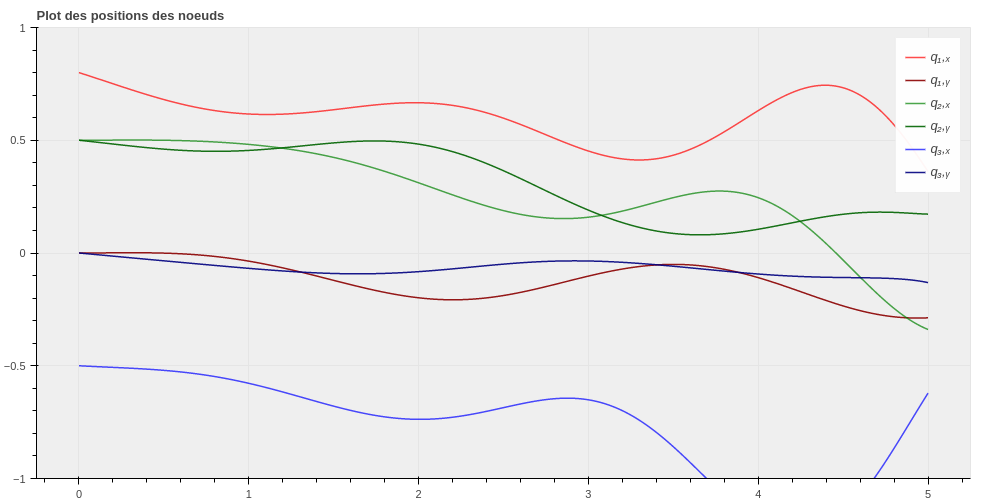
\includegraphics[width=\textwidth]{PlotDeplacement2D-1-Conv.png}
        \caption{Simulation des positions des noeuds.}
        \label{fig:dep}
    \end{subfigure}
%     \hfill
    \begin{subfigure}[b]{0.7\textwidth}
        \centering
        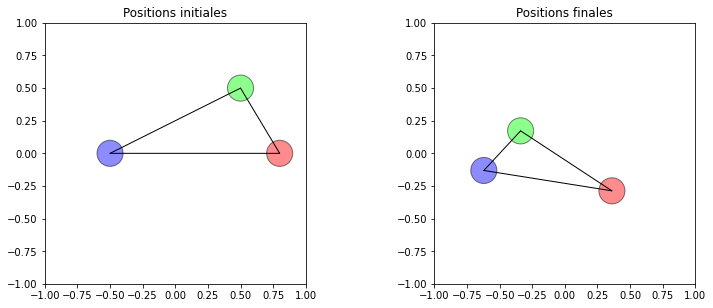
\includegraphics[width=\textwidth]{PositionInitFinales.png}
        \caption{Illustration des positions initiales et finales des neouds.}
        \label{fig:pos}
    \end{subfigure}
    \caption{Simulation du système \ref{eq:systeme2D} par un schéma d'Euler explicite avec $T = 4$. La couleurs rouge repésente le noeud $\bvec{q}_1$, le vert le noeud $\bvec{q}_2$, le blue le $\bvec{q}_3$. Les paramètres utilisés ici sont les suivants: $m=6.2$, $k=23.3$, $\mu=3$; à l'instant initiale, les trois noeuds perturbés avec des vitesses d'intensité respectives $v_1=0.3$, $v_2=0.1$, et $v_3=0.1$. Par rapport à l'axe des abcisses, ces vitesses ont sont orintées respectivement de $\theta_1=180^\circ$, $\theta_2=270^\circ$, et $\theta_3=240^\circ$ (voir \texttt{code/simu2D/Deplacement2D-1.ipynb}).}
    \label{fig:PlotDeplacement2D1Conv}
\end{figure}


\begin{figure}[!h]
    \centering
    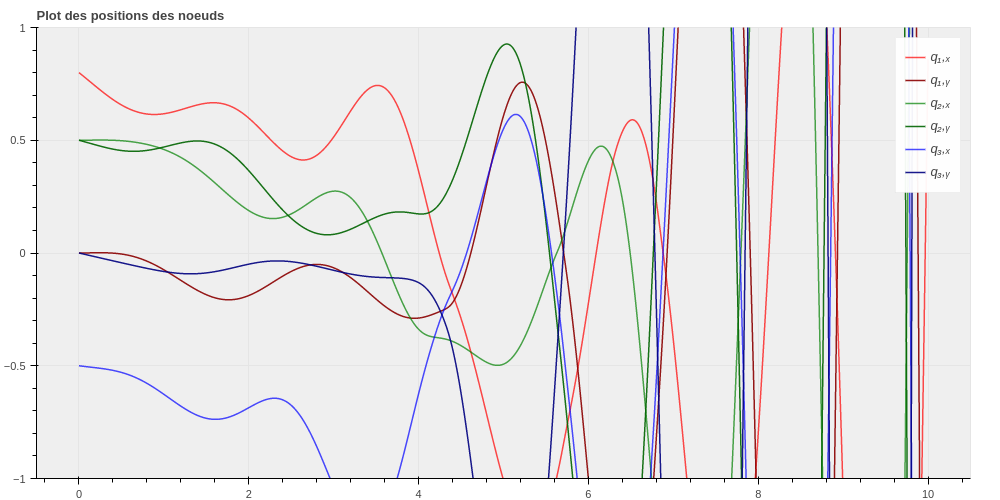
\includegraphics[width=0.7\textwidth]{PlotDeplacement2D-1-NonConv.png}
    \caption{Simulation du système \ref{eq:systeme2D} par un schéma d'Euler explicite avec $T = 10$. Cette figure utilise les même paramtètres que la \cref{fig:PlotDeplacement2D1Conv}. On observe ici une divergence totale du système.}
    \label{fig:PlotDeplacement2D1NonConv}
\end{figure}

Les \cref{fig:PlotDeplacement2D1Conv,fig:PlotDeplacement2D1NonConv} permettent de constater que le schéma d'Euler explicite (peu importe son pas de temps), n'est pas adapté à ce problème. Nous étudierons donc d'autres alternatives. 

 
\paragraph{Simulation à l'aide des fonction de la librarie Scipy.} À travers ses fonction telle que \texttt{odeint} et $\verb|solve_ivp|$, \texttt{Scipy} offre une solution robuste et élégante pour simuler les systèmes d'ODE de la forme $Y' = AY$.


 




\subsubsection{Modélisation du contact entre deux floes}

Les floes de glace $\Omega_k$ et $\Omega_l$ sont modélisés par des systèmes masse-ressort (à grande raideur). Pour l'instant, nous considérons une moélisation simplifiée qui assimile un floe à un système de (trois) masses reliés par des ressorts (de constante de raideur $k$), et par des dispositifs visqueux de constante $\mu$.
Nous désignerons par $n+1$ le nombre total de noeuds du floe $\Omega_k$, chaque noeud ayant pour masse $m$. De facon similaire, on définit les constantes $k'$, $\mu'$, $n'+1$, $m'+1$ pour le floe $\Omega_l$. Les positions des noeds de $\Omega_k$ seront noté $(q_i)_{0\leq i\leq n}$, tandis que ceux de $\Omega_l$ seront notés $(p_i)_{0 \leq i\leq n'}$ (voir \cref{fig:contactmanuel}). 

\begin{figure}[!h]
    \centering
    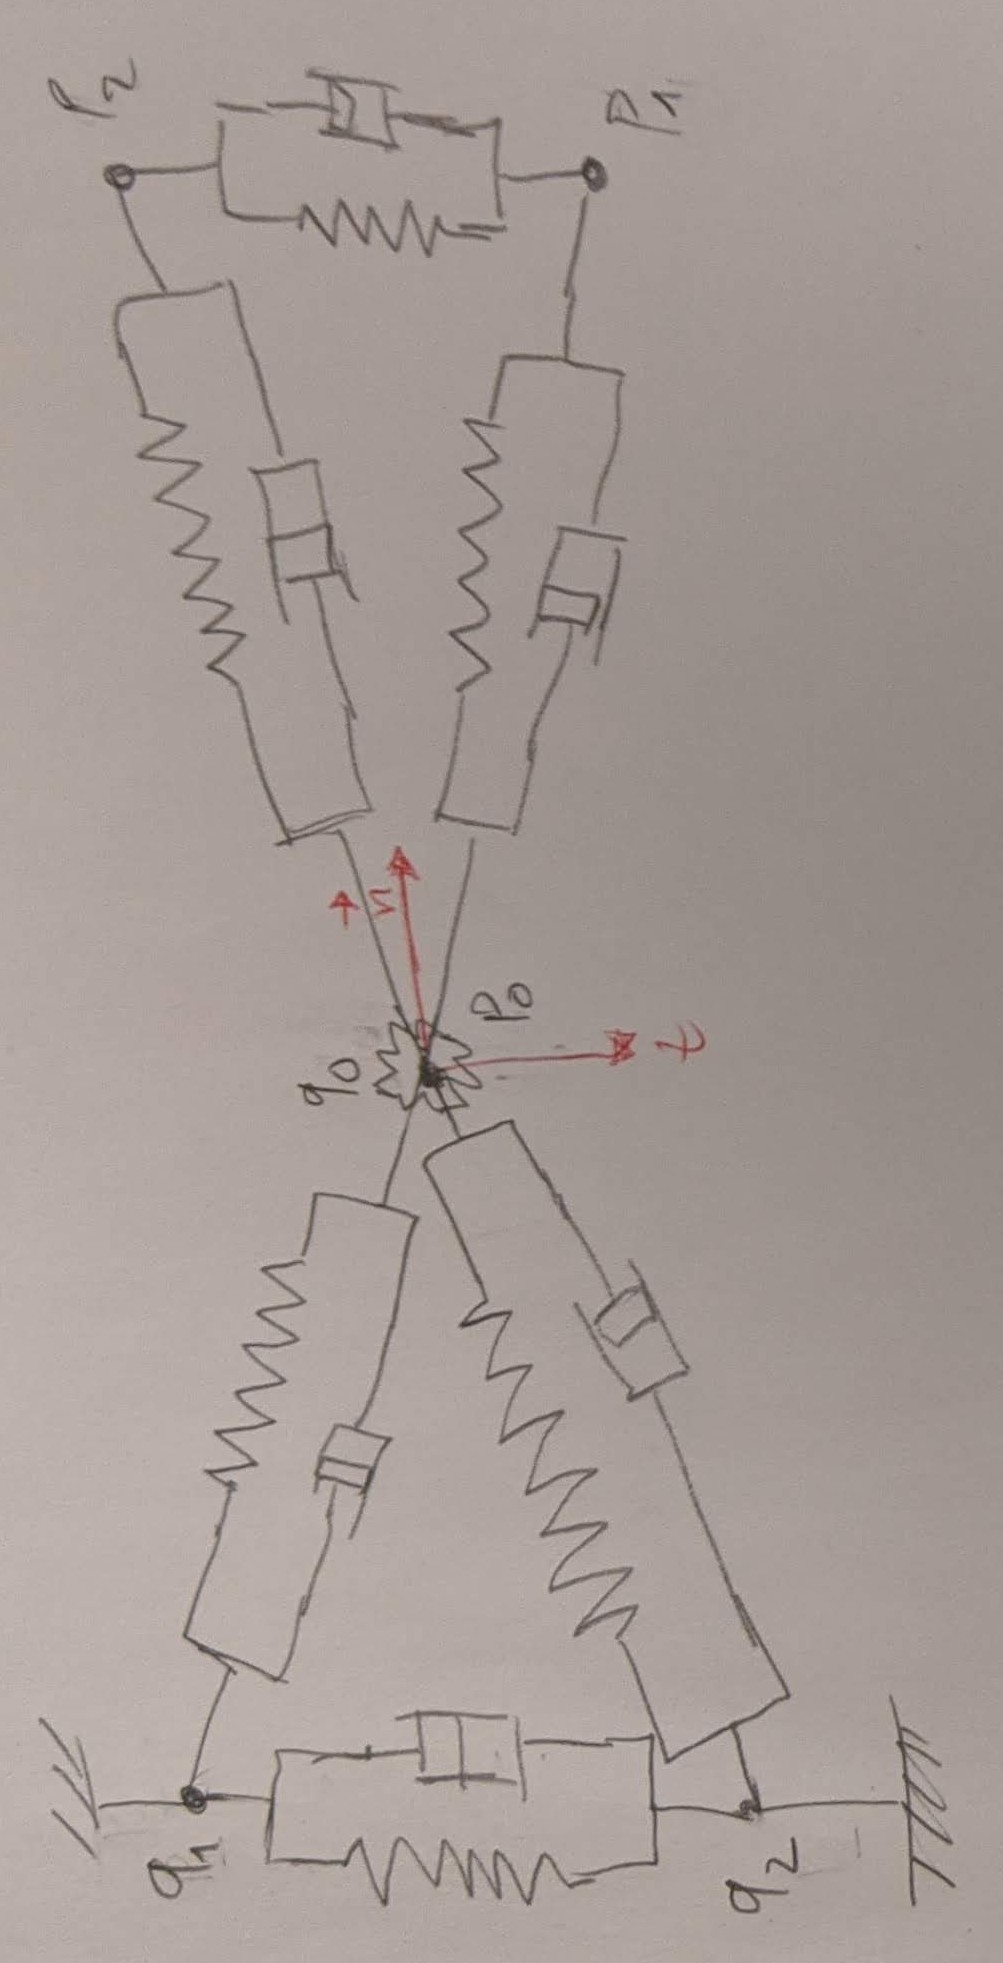
\includegraphics[width=0.3\textwidth, angle=-90]{ContactManuel.jpg}
    \caption{Contact entre deux floes aux points $p_0 = q_0$.}
    \label{fig:contactmanuel}
\end{figure}

\noindent On définit la matrice de contact $C$...(voir these Dimitri), et $L_{0j}$.. et $u_{0j}$ ..

\noindent Comme présenté dans les travaux \parencite[p.186]{balasoiu2020halthesis}, le système différentiel qui modélise la percussion s’écrit comme le couplage de deux sous-systèmes. Le premier, dit système intérieur (SI), est à évolution rapide et modélise la propagation des ondes élastiques dans le système masse-ressort. Ici, nous dérivons facilement et réutilisont le SI comme présenté par \citeauthor{balasoiu2020halthesis}. Le second, dit système extérieur (SE), est à évolution lente et modélise la pénétration de l’objet solide dans le système masse-ressorts. Pour dériver le SE sur le floe $\Omega_k$, nous écrivons l'équation de Newton-Euler linéaire\footnote{La rotation du point matériel $q_0$ n'est pas prise en compte ici, d'où l'abscence de l'équation de Newton-Euler angulaire.} au point de contact $q_0$:
\begin{align}  \label{eq:SE}
m \ddot{\bvec{q}}_0 = \bvec{F}_0 + \bvec{F}^c_0 \,,
\end{align}
où 
\begin{align}  \label{eq:F0}
    \bvec{F}_0 = \sum_{j=0}^{n}C_{0j} \left[  \underbrace{k \left( \Vert \bvec{q}_j - \bvec{q}_0 \Vert - L_{0j} \right) \bvec{u}_{0j}}_{\text{Force de rappel}} - \underbrace{\mu \left\langle \bvec{\dot{q}}_j - \bvec{\dot{q}}_0\,, \bvec{u}_{0j}  \right\rangle  \bvec{u}_{0j}}_{\text{Force de dissipation}}  \right] \,,
\end{align}
représente la somme des forces de reaction et de disssipation exercées par le ressort et le dispositif visqueux sur le noeud $q_0$ ; et $\bvec{F}^c_0(t)$ la force de contact durant la collison entre les deux particules. En supposnat qu'il existe un repère de contact $\mathcal{R}^c = \{ q_0, \bvec{n}, \bvec{t} \}$ associé au floe $\Omega_k$ (voir \cref{fig:contactmanuel}), on peut écrire, pour $(\lambda, \beta) \in \Rdeux$ :
\begin{align}  \label{eq:F0c}
    \bvec{F}_0^c = \lambda \bvec{n} + \beta \bvec{t} \,.
\end{align}
Le système intérieur (SE) s'obtient facilement en combinant les équations \cref{eq:SE,eq:F0,eq:F0c}. Le système intérieur (SI) s'obtient lui (pour les autres noeuds du réseau) en y supprimant la force de contact. On obtient au final:
\begin{align} \tag{$E$} \label{eq:e}
\begin{dcases}
    m \ddot{\bvec{q}}_0 = \bvec{F}_0 + \bvec{F}^c_0  \,, &\qquad \text{(SE)} \\
    m \ddot{\bvec{q}}_i = \bvec{F}_i   \,, \quad \quad \quad \forall 1 \leq i \leq n \,. &\qquad \text{(SI)}
\end{dcases}
\end{align}
En ce qui concerne le floe $\Omega_l$, nous procédons de facons similaire et appliqons la 3ème loi de Newton (action-réaction) pour obtenir le système:
\begin{align} \tag{$E'$} \label{eq:eprime}
\begin{dcases}
    m' \ddot{\bvec{p}}_0 = \bvec{F}^{'}_0 - \bvec{F}^c_0  \,, &\qquad \text{(SE)} \\
    m' \ddot{\bvec{p}}_i = \bvec{F}^{'}_i   \,, \quad \quad \quad \forall 1 \leq i \leq n' \,, &\qquad \text{(SI)}
\end{dcases}
\end{align}
où $(\bvec{F}^{'}_i)_{0 \leq i \leq n'}$ sont définis de facon similaire à $\bvec{F}_0$ (voir \cref{eq:F0}):
\begin{align}
    \bvec{F}'_i = \sum_{j=i}^{n'}C_{ij} \left[ k' \left( \Vert \bvec{p}_j - \bvec{p}_i \Vert - L'_{ij} \right) \bvec{u'}_{ij} - \mu' \left\langle \bvec{\dot{p}}_j - \bvec{\dot{p}}_i\,, \bvec{u}'_{ij}  \right\rangle  \bvec{u}'_{ij}  \right] \,.
\end{align}

\noindent Ensuite, on additionne membre à membre les équations des systèmes extérieurs (SE) de \cref{eq:e,eq:eprime} pour éliminer la force de contact. On obtient:
\begin{align}
m \ddot{\bvec{q}}_0 + m' \ddot{\bvec{p}}_0 = \bvec{F}_0 + \bvec{F}^{'}_0 \,.
\end{align}
Remarquons que les positions relatives des noeuds $\bvec{q}_0$ et $\bvec{p}_0$ restent inchangées durant la collision. A l'instant initial, on note donc $\Delta_0 = \bvec{q}_0(0) - \bvec{p}_0(0)$; ainsi : 
\begin{align}
\forall t \in \mathbb{R}^+ \,, \quad \bvec{q}_0(t) - \bvec{p}_0(t) = \Delta_0\,.
\end{align}
Nous avons aisni obtenu les $n+n'+2$ équations nécessaire pour que notre problème de percussion soit bien posé. Elles sont :
\begin{align} \tag{$\mathcal{P}$} \label{eq:problemeP}
\begin{dcases}
    m \ddot{\bvec{q}}_0 + m' \ddot{\bvec{p}}_0 = \bvec{F}_0 + \bvec{F}^{'}_0  \,, &\qquad \text{(SE)} \\
    \bvec{q}_0 - \bvec{p}_0 = \Delta_0 \,, &\qquad \text{(SE)} \\
    m \ddot{\bvec{q}}_i = \bvec{F}_i   \,, \quad \quad \quad \forall 1 \leq i \leq n \,. &\qquad \text{(SI)} \\
    m' \ddot{\bvec{p}}_i = \bvec{F}^{'}_i   \,, \quad \quad \quad \forall 1 \leq i \leq n' \,, &\qquad \text{(SI)}
\end{dcases}
\end{align}

Ensuite, il nous faut introduire des conditions portant sur la conservation de l'énergie, et la condition de non-interpénétration de Signorini\dots







% \section{Les apports du stage}

%\begin{itemize}
%    \item L' utilisation de TIKZ
%\end{itemize}